
%%%%%%%%%%%%%%%%%%%%%%%%%%%%%%%%%%%%%%%%%%%%%%%%%%%%%%%%%%%%%%%%%%%%%%%%%%%%%%%%%%%%%%%%%%%%%%%%%%%%%%%%%%%%%%
% Article:
% Bootstrap Inference for the Area Under the ROC Curve
% Simulations
%%%%%%%%%%%%%%%%%%%%%%%%%%%%%%%%%%%%%%%%%%%%%%%%%%%%%%%%%%%%%%%%%%%%%%%%%%%%%%%%%%%%%%%%%%%%%%%%%%%%%%%%%%%%%%%

\section{Simulation Evidence} \label{sec:sims}



\subsection{Data Generating Process}

%Structure of Simulation
%\begin{itemize}
%    \item Regime-switching model
%    \begin{itemize}
%        \item 2 states, high- and low-AUROC regimes, equally likely
%        \item past regimes known, future unknown
%    \end{itemize}
%    \item Measure AUROC from both regimes
%    \item Measure distance between distributions in regimes
%    \item Calculate extreme AUROC values that correspond to movements away from full dataset, using distances between observed distributions
%\end{itemize}

This next section presents the results of some simulation exercises to demonstrate the effectiveness of the statistical methodology, with $1,000$ replications in each.
%
Each exercise will show two types of coverage rates for the AUROC.
%
The first type, following the standard definition, are defined as the proportion of confidence intervals that contain the true values of the AUROC.

Confidence intervals represent the range of values such that, when calculated in such a way, would be expected to contain the true value of the parameter in question.
The width of such an interval is calculated in a way that only accounts for the sampling variation.

The statistics that are labeled as correct forecast rates are the proportion of forecast intervals that contain the estimated values of the AUROC that are realized from the data generating process.
These rates account for both the variation in the sample from a fixed population and the variation in the data generating process, which is described next.



The data generating process is a two-state regime-switching model with a bi-normal classification model in each state.
That is, with equal probability, a drawing is made from the high ($H$) and low ($L$) regimes.
Then a sample of data is drawn from the selected distribution, with true AUROC values of $A_L$ in the low state and $A_H$ in the high state.
In each state, the drawing is made from a bi-normal classification model.
This model is made up of a drawing from a pair of normal distributions.
The observations corresponding to positive events are drawn from one normal distribution and those corresponding to the negative distribution are drawn from another.
There are $1,000$ negative observations and $100$ negative observations.
Both normal distributions have a standard deviation of $1/\sqrt{2}$, which implies a pooled variance of $1$.
The classification variables corresponding to negative events in the bi-normal model have mean zero, while those linked to positive events have mean in accordance with the specified AUROC values.

The simulation is divided into four sections.
In the first, the AUROC parameters are set at $A_L = 0.68$ and $A_H = 0.72$.
In the second, the parameters are farther apart at $A_L = 0.65$ and $A_H = 0.75$.
In the third, the AUROC parameters take on higher values at $A_L = 0.75$ and $A_H = 0.80$.
The fourth simulation has no regime-switching behavior, with AUROC in both states set to $0.70$.


\subsection{Alternative Methods of Inference}

%% Moved to Intro.
%To explain the other lines in the analysis.
%
%Brief description in intro.
%Equations shown here for detail.
%\begin{itemize}
%
%    \item Theoretical confidence bounds.
%
%    For binormal ROC, refer to \citet{demidenko2012}.
%    For biexponential ROC, refer to \citet{hanleymcneil1982} for standard errors.
%
%    \item Empirical $z$-statistic.
%
%    \item Upper bound of variance, as described in \citet{birn1957} and \citet{vandan1915} (Note: Something wrong with the date. Check reference.).
%
%    \item Fixed error rate (\citet{cortezMohri2004}).
%
%\end{itemize}
%
%
%Confidence Intervals in Literature
%\begin{itemize}
%
%    \item Parametric models:
%    \begin{itemize}
%        \item Binormal model: $[\Phi(\tilde{z}_{\alpha/2}), \Phi(\tilde{z}_{1-\alpha/2})]$
%        \item Biexponential model: $[\hat{A} \pm  z_{1-\alpha/2} \hat{\sigma}_A]$, with \\
%        $\sigma^2_A = \frac{1}{mn} \{ A(1 - A) + (n - 1)(P_{yyx} - A^2) + (m - 1)(P_{yxx} - A^2) \}$,
%        $P_{yyx} = A/(2-A)$, $P_{yxx} = 2A^2/(1+A)$
%    \end{itemize}
%
%    \item Empirical distribution: $P_{yyx} = \frac{1}{mnn} \sum_i \sum_j \sum_k I_{\left\{ y_j > x_i \cap y_k > x_i \right\}}$ \\
%    $\qquad\qquad\qquad\qquad$ and $P_{yyx} = \frac{1}{mmn} \sum_i \sum_j \sum_k I_{\left\{ y_j > x_i \cap y_j > x_k \right\}}$
%
%    \item Upper bound of variance: $\sigma^2_{max} = \frac{A(1-A)}{\min\{ m, n \}} \left( \leq \frac{1}{4 \min\{ m, n \} } \right) $
%
%    \item Fixed error rate: (next)
%
%\end{itemize}




The forecast intervals produced in this analysis are compared to several other intervals produced in the literature.
The first case takes advantage of the knowledge that the model is bi-normal.
In this special case, the AUROC reduces to the normal CDF evaluated at the statistic for testing the hypothesis of equality of the means of the normal distributions.
The confidence interval is calculated by evaluating the CDF at two quantiles of the test statistic, with an adjustment for the nonlinear transformation, by way of the delta method.
The expression is described in \citet{demidenko2012}.

The second example is a more flexible method, in which the confidence interval is constructed using an estimate of the variance of AUROC.
The expression for this estimate is calculated in \citet{hanleymcneil1982}, using the methods in \citet{proc2011}, following the computational strategy in \citet{sunxu2014}.
%
\begin{equation}
    \sigma^2_A = \frac{1}{mn} \{ A(1 - A) + (n - 1)(P_{yyx} - A^2) + (m - 1)(P_{yxx} - A^2) \}
\end{equation}
%
The terms $P_{yyx}$ and $P_{yxx}$ in the above are defined as
%
\begin{equation}
    P_{yyx} = \frac{1}{mnn} \sum_i \sum_j \sum_k I_{\left\{ y_j > x_i \cap y_k > x_i \right\}}
    \qquad
    P_{yxx} = \frac{1}{mmn} \sum_i \sum_j \sum_k I_{\left\{ y_j > x_i \cap y_j > x_k \right\}}.
\end{equation}
%
The expressions are higher-order terms of the calculation of the AUROC itself.
They are evaluated by drawing three observations by drawing two from either the positive or negative classification variables and one from the other.
The values of $P_{yyx}$ and $P_{yxx}$ are the probabilities that both such pairs are correctly ordered.

The third method is calculated with a bootstrap technique, with $399$ bootstrap replications for each confidence interval.
These are calculated using the approach in \citet{proc2011}, and is computed by drawing realizations of the observations, with replacement, and calculating the AUROC.
The confidence intervals are then computed by using the upper and lower quantiles.

Taking an upper bound on the variance of the AUROC produces a more conservative estimate of a range that should contain the true values.
The approach is described in \citet{birn1957} and \citet{vandan1915} and has the following form.
%
\begin{equation}
    \sigma^2_{max} = \frac{A(1-A)}{\min\{ m, n \}}
    \left( \leq \frac{1}{4 \min\{ m, n \} } \right)
\end{equation}
%

% \textbf{hourglass figure:}

% {\Large Insert hourglass figure of AUROC interval possibilities for distributions a specific distance away.}

% Overall, I am measuring the amount of variation that would go undetected by a distance metric from the reference distribution.
% Here, I am showing a continuum of variation, indexed by each particular distance from the reference distribution.




%%%%%%%%%%%%%%%%%%%%%%%%%%%%%%%%%%%%%%%%%%%%%%%%%%%%%%%%%%%%%%%%%%%%%%%%%%%%%%%%%%%%%%%%%%%%%%%%%%%%%%%%%%%%%%%


\begin{figure}[h!]

\begin{center}

    \caption{Forecast and Confidence Intervals} \label{fig:Forecast1}

        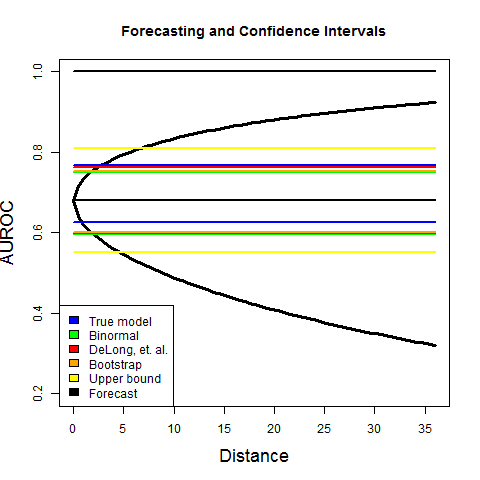
\includegraphics[scale=  0.75]{Figs/Forecast/Forecast_int_1.png}



\end{center}

    \footnotesize

        \textbf{Forecast and Confidence Intervals:}
        Forecast intervals are produced as a function of distance from the sample distribution (black curves).
        Under the null hypothesis of a fixed sampling distribution, distance would follow a $\chi^2$ distribution with $9$ degrees of freedom.
        Confidence intervals are shown for the AUROC for a variety of methods, at the $95\%$ confidence level.
        % 
        As the forecast intervals are scaled by the estimate of distance, it is possible that the intervals will expand to account for added variation, while others remain fixed. 
        %
        The sample is drawn from a bi-normal distribution with a true AUROC of $0.70$, with positive classification variable distribution with a mean of $0$ and standard deviation of $1/\sqrt{2}$, and negative positive classification variable distribution with a mean of $0.5244$ and standard deviation of $1/\sqrt{2}$.
        Sample size is $1,100$ in total, with $1,000$ negative observations and $100$ positive observations.

% Terms in $KLD(\textcolor{blue}{f_1}, \textcolor{red}{f_2})
%  = \sum_{k = 1}^{K} \left\{ \textcolor{magenta}{\big( f_1(t_k) - f_2(t_k) \big)}
%         \textcolor{orange}{\log \left( \frac{f_1(t_k)}{f_2(t_k)} \right)} \right\}$

\end{figure}


%%%%%%%%%%%%%%%%%%%%%%%%%%%%%%%%%%%%%%%%%%%%%%%%%%%%%%%%%%%%%%%%%%%%%%%%%%%%%%%%%%%%%%%%%%%%%%%%%%%%%%%%%%%%%%%



Figure \ref{fig:Forecast1} shows confidence intervals for the AUROC for the above list of methods, at the $95\%$ confidence level.
It is contrasted against the forecast intervals that are produced as a function of distance from the sample distribution, represented by the black curves.
% Under the null hypothesis of a fixed sampling distribution, distance would follow a $\chi^2$ distribution with $9$ degrees of freedom.
%
As the forecast intervals are scaled by the estimate of distance, it is possible that the intervals will expand to account for added variation, while others remain fixed.
%
This allows for the potential for variation that erodes the coverage rates of the fixed intervals, while the forecast intervals are flexible to accommodate such variation.
% Forecast intervals as a function of distance from the sample distribution (black curves).
% These are contrasted against a series of $95\%$ confidence intervals for the AUROC for a variety of methods.
%
% Under the null hypothesis of a fixed sampling distribution, distance would follow a $\chi^2$ distribution with $9$ degrees of freedom.





Finally, one more approach is presented in \citet{cortezMohri2004}, in which the confidence interval is parameterized as a function of the anticipated error rate.
In this way, the variance can be expanded beyond the distribution represented in the sample.
It is also reeled in from the upper bound drawn up by all possible distributions that could occur.
This novel approach is excluded from the simulation but is mentioned since it allows for the intervals to be scaled by a parameter chosen by the modeler, as is done in the simulations that follow.




%  with $399$ bootstrap replications for bootstrap confidence intervals.

%    \item Measure AUROC from both regimes
%    \item Measure distance between distributions in regimes
%    \item Calculate extreme AUROC values that correspond to movements away from full dataset, using distances between observed distributions


Under each of these simulations, the sample is drawn from the regime-switching model, with labels to denote the subsamples by regime.
%
This can be interpreted as a form of seasonality that is known to the researcher, except that the features of the sample are unknown.
%
Another interpretation is that the modeler can propose a model for the distributions in each regime.
%
This approach was not followed here, as it is intended to apply without parametric model specifications. 
% 
This sort of simulation employed here is designed as a simple approach to modeling the time-varying nature of the data generating process in a way that can be easily understood. 
%
% This allows for

\subsection{Coverage Rates}


Across the four models, the performance of the methods follows a particular pattern.
In the first case, with $A_L = 0.68$ and $A_H = 0.72$, there is a modest amount of variability in the model, so the competing methods still produce reasonable coverage rates greater than $80\%$.
Performance drops for forecast accuracy, with the specified intervals containing future estimates roughly two thirds of the time.
The distance-based forecast method produces coverage greater than $90\%$ in all cases.

In the next model, with $A_L = 0.65$ and $A_H = 0.75$, the true AUROC has much more variability.
The other techniques are unable to capture this variation and coverage rates are much lower.
In the third case, with $A_L = 0.75$ and $A_H = 0.80$, the true variability is lower, but the variances within each of the first three standard methods is based on a leading term of the form $A(1-A)$, which is lower for populations with AUROC in this higher range.
For this reason, these techniques underestimate the variance of the estimates and produce lower coverage rates.
The exception is the method that uses an upper bound on the variance, which produces higher coverage rates with the wider intervals.
In the fourth case, the AUROC is a fixed $0.70$ and the competing methods fare much better.
Under the Bi-normal, DeLong and Bootstrap approaches, the model is correctly specified and the statistics show results close to the nominal $95\%$ coverage rates.


Consider the results along the list of modeling approaches considered.
The AUROC is estimated from the full sample and a confidence interval is constructed around this value under each of the approaches listed above.
To this list, the forecast intervals defined in this paper are proposed as an alternative.
These are constructed by calculating the average distance $\bar{D}$ between the subsamples and the full samples.
These distances are used to shift the distributions of classification variables to generate the farthest values of AUROC that can be generated with a distribution of distance $\bar{D}$ from the sample observed.
The extreme values of AUROC define the bounds of the forecast interval.

Overall, the distance-based forecasting method produces acceptable performance in all cases, as a method for constructing forecast intervals.
The closest competitor is the technique using an upper bound on the variance, which is enough to capture the variability in estimated AUROC, at least for the cases with less variability.
The distance-based forecast method is the only one that scales the width of the interval to account for additional variation.



% \subsection{Coverage Rates}

%Tables for three cases.
%Two variants on regime-switching model.
%One for a fair comparison.



%%%%%%%%%%%%%%%%%%%%%%%%%%%%%%%%%%%%%%%%%%%%%%%%%%%%%%%%%%%%%%%%%%%%%%%%%%%%%%%%%%%%%%%%%%%%%%%%%%%%%%%%%%%%%%%


% \begin{figure}[h!]
\begin{table}[h!]

\begin{center}

    % \hline
    \caption{Rates of Coverage and Correct Forecasts} \label{fig:Coverage1}

    % \hline
    \begin{tabular}{l l c c }

    True Values & Method & Coverage Rate & Correct Forecast Rate \\

    \hline

    %[1] "Coverage rates for n = 1100, A_L = 0.680000, A_H = 0.720000"
%               method coverage  forecast
%    1:      Bi-normal   0.8265 0.6612295
%    2: DeLong et. al.   0.8395 0.6689495
%    3:      Bootstrap   0.8310 0.6616050
%    4:    Upper Bound   0.9885 0.9074855
%    5:       Forecast   0.9955 0.9600615

$A_L = 0.68$, &
          Bi-normal &  0.8265 & 0.6612 \\
$A_H = 0.72$ &
     DeLong et. al. &  0.8395 & 0.6689 \\
 &         Bootstrap &  0.8310 & 0.6616 \\
 &       Upper Bound &  0.9885 & 0.9074 \\
 &          Forecast &  0.9955 & 0.9600 \\


    \hline

%    [1] "Coverage rates for n = 1100, A_L = 0.650000, A_H = 0.750000"
%           method coverage  forecast
%    1:      Bi-normal   0.2360 0.3427380
%    2: DeLong et. al.   0.2470 0.3515930
%    3:      Bootstrap   0.2455 0.3453490
%    4:    Upper Bound   0.7725 0.6615905
%    5:       Forecast   0.9795 0.9259675

$A_L = 0.65$, &
          Bi-normal &  0.2360 & 0.3427 \\
$A_H = 0.75$ &
     DeLong et. al. &  0.2470 & 0.3515 \\
 &         Bootstrap &  0.2455 & 0.3453 \\
 &       Upper Bound &  0.7725 & 0.6615 \\
 &          Forecast &  0.9795 & 0.9259 \\


    \hline

%    [1] "Coverage rates for n = 1100, A_L = 0.750000, A_H = 0.800000"
%           method coverage  forecast
%    1:      Bi-normal   0.6805 0.5912520
%    2: DeLong et. al.   0.6845 0.5979860
%    3:      Bootstrap   0.6730 0.5889715
%    4:    Upper Bound   0.9665 0.8654290
%    5:       Forecast   0.9940 0.9451650

$A_L = 0.75$, &
          Bi-normal &  0.6805 & 0.5912 \\
$A_H = 0.80$ &
     DeLong et. al. &  0.6845 & 0.5979 \\
 &         Bootstrap &  0.6730 & 0.5889 \\
 &       Upper Bound &  0.9665 & 0.8654 \\
 &          Forecast &  0.9940 & 0.9451 \\

    \hline

%    [1] "Coverage rates for n = 1100, A_L = 0.700000, A_H = 0.700000"
%           method coverage  forecast
%    1:      Bi-normal    0.951 0.7402125
%    2: DeLong et. al.    0.944 0.7477020
%    3:      Bootstrap    0.941 0.7386815
%    4:    Upper Bound    1.000 0.9464325
%    5:       Forecast    0.999 0.9702450

$A_L = 0.70$, &
          Bi-normal  &  0.951 & 0.7402 \\
$A_H = 0.70$ &
     DeLong et. al.  &  0.944 & 0.7477 \\
 &         Bootstrap  &  0.941 & 0.7386 \\
 &       Upper Bound  &  1.000 & 0.9464 \\
 &          Forecast  &  0.999 & 0.9702 \\

    \hline

    \end{tabular}

    % \hline

\end{center}

    \footnotesize

        \textbf{Rates of Coverage and Correct Forecasts:}
        Coverage rates are the proportion of confidence intervals that contain the true values of the AUROC.
        Correct forecast rates are the proportion of confidence intervals that contain the estimated values of the AUROC.
        Number of replications is $1,000$ for all models, with $399$ bootstrap replications for bootstrap confidence intervals.
        Data generating process is a two-state regime-switching model with a bi-normal classification model in each state,
        with true AUROC values of $A_L$ in the low state and $A_H$ in the high state.
        % Bi-normal models have standard deviations of $1/sqrt{2}$.
        % Positive distributions have


    % \hline



% \end{figure}
\end{table}


%%%%%%%%%%%%%%%%%%%%%%%%%%%%%%%%%%%%%%%%%%%%%%%%%%%%%%%%%%%%%%%%%%%%%%%%%%%%%%%%%%%%%%%%%%%%%%%%%%%%%%%%%%%%%%%



%
%%%%%%%%%%%%%%%%%%%%%%%%%%%%%%%%%%%%%%%%%%%%%%%%%%%%%%%%%%%%%%%%%%%%%%%%%%%%%%%%%%%%%%%%%%%%%%%%%%%%%%%%%%%%%%%

Coverage Rates \\
True values: $A_L = 0.68, A_H = 0.72$

\begin{figure}[h!]

\begin{center}

    % \hline
    % \caption{Rates of Coverage and Correct Forecasts ($A_L = 0.68, A_H = 0.72$)} \label{fig:Coverage1}

    % \hline
    \begin{tabular}{l c c }

    Method & Coverage Rate & Correct Forecast Rate \\

    \hline

    %[1] "Coverage rates for n = 1100, A_L = 0.680000, A_H = 0.720000"
%               method coverage  forecast
%    1:      Bi-normal   0.8265 0.6612295
%    2: DeLong et. al.   0.8395 0.6689495
%    3:      Bootstrap   0.8310 0.6616050
%    4:    Upper Bound   0.9885 0.9074855
%    5:       Forecast   0.9955 0.9600615


          Bi-normal &  0.8265 & 0.6612 \\
     DeLong et. al. &  0.8395 & 0.6689 \\
          Bootstrap &  0.8310 & 0.6616 \\
        Upper Bound &  0.9885 & 0.9074 \\
           Forecast &  0.9955 & 0.9600 \\


    \hline

    \end{tabular}

    % \hline

\end{center}

%    \footnotesize
%
%        \textbf{Rates of Coverage and Correct Forecasts:}
%        Coverage rates are the proportion of confidence intervals that contain the true values of the AUROC.
%        Correct forecast rates are the proportion of confidence intervals that contain the estimated values of the AUROC.
%        Number of replications is $1,000$ for all models, with $399$ bootstrap replications for bootstrap confidence intervals.
%        Data generating process is a two-state regime-switching model with a bi-normal classification model in each state,
%        with true AUROC values of $0.68$ in the low state and $0.72$ in the high state.
%        % Bi-normal models have standard deviations of $1/sqrt{2}$.
%        % Positive distributions have


    % \hline



\end{figure}


%%%%%%%%%%%%%%%%%%%%%%%%%%%%%%%%%%%%%%%%%%%%%%%%%%%%%%%%%%%%%%%%%%%%%%%%%%%%%%%%%%%%%%%%%%%%%%%%%%%%%%%%%%%%%%%


%
%%%%%%%%%%%%%%%%%%%%%%%%%%%%%%%%%%%%%%%%%%%%%%%%%%%%%%%%%%%%%%%%%%%%%%%%%%%%%%%%%%%%%%%%%%%%%%%%%%%%%%%%%%%%%%%


\begin{figure}[h!]

\begin{center}

    % \hline
    \caption{Rates of Coverage and Correct Forecasts ($A_L = 0.65, A_H = 0.75$)} \label{fig:Coverage1}

    % \hline
    \begin{tabular}{l c c }

    Method & Coverage Rate & Correct Forecast Rate \\

    \hline
    
%    [1] "Coverage rates for n = 1100, A_L = 0.650000, A_H = 0.750000"
%           method coverage  forecast
%    1:      Bi-normal   0.2360 0.3427380
%    2: DeLong et. al.   0.2470 0.3515930
%    3:      Bootstrap   0.2455 0.3453490
%    4:    Upper Bound   0.7725 0.6615905
%    5:       Forecast   0.9795 0.9259675


          Bi-normal &  0.2360 & 0.3427 \\
     DeLong et. al. &  0.2470 & 0.3515 \\
          Bootstrap &  0.2455 & 0.3453 \\
        Upper Bound &  0.7725 & 0.6615 \\
           Forecast &  0.9795 & 0.9259 \\


    \hline

    \end{tabular}

    % \hline

\end{center}

    \footnotesize

        \textbf{Rates of Coverage and Correct Forecasts:}
        Coverage rates are the proportion of confidence intervals that contain the true values of the AUROC.
        Correct forecast rates are the proportion of confidence intervals that contain the estimated values of the AUROC.
        Number of replications is $1,000$ for all models, with $399$ bootstrap replications for bootstrap confidence intervals.
        Data generating process is a two-state regime-switching model with a bi-normal classification model in each state,
        with true AUROC values of $0.65$ in the low state and $0.75$ in the high state.
        % Bi-normal models have standard deviations of $1/sqrt{2}$.
        % Positive distributions have


    % \hline



\end{figure}


%%%%%%%%%%%%%%%%%%%%%%%%%%%%%%%%%%%%%%%%%%%%%%%%%%%%%%%%%%%%%%%%%%%%%%%%%%%%%%%%%%%%%%%%%%%%%%%%%%%%%%%%%%%%%%%


%
%%%%%%%%%%%%%%%%%%%%%%%%%%%%%%%%%%%%%%%%%%%%%%%%%%%%%%%%%%%%%%%%%%%%%%%%%%%%%%%%%%%%%%%%%%%%%%%%%%%%%%%%%%%%%%%


\begin{figure}[h!]

\begin{center}

    % \hline
    \caption{Rates of Coverage and Correct Forecasts ($A_L = 0.75, A_H = 0.80$)} \label{fig:Coverage1}

    % \hline
    \begin{tabular}{l c c }

    Method & Coverage Rate & Correct Forecast Rate \\

    \hline
    
%    [1] "Coverage rates for n = 1100, A_L = 0.750000, A_H = 0.800000"
%           method coverage  forecast
%    1:      Bi-normal   0.6805 0.5912520
%    2: DeLong et. al.   0.6845 0.5979860
%    3:      Bootstrap   0.6730 0.5889715
%    4:    Upper Bound   0.9665 0.8654290
%    5:       Forecast   0.9940 0.9451650
    
    
          Bi-normal &  0.6805 & 0.5912 \\
     DeLong et. al. &  0.6845 & 0.5979 \\
          Bootstrap &  0.6730 & 0.5889 \\
        Upper Bound &  0.9665 & 0.8654 \\
           Forecast &  0.9940 & 0.9451 \\

    \hline

    \end{tabular}

    % \hline

\end{center}

    \footnotesize

        \textbf{Rates of Coverage and Correct Forecasts:}
        Coverage rates are the proportion of confidence intervals that contain the true values of the AUROC.
        Correct forecast rates are the proportion of confidence intervals that contain the estimated values of the AUROC.
        Number of replications is $1,000$ for all models, with $399$ bootstrap replications for bootstrap confidence intervals.
        Data generating process is a two-state regime-switching model with a bi-normal classification model in each state,
        with true AUROC values of $0.75$ in the low state and $0.80$ in the high state.
        % Bi-normal models have standard deviations of $1/sqrt{2}$.
        % Positive distributions have


    % \hline



\end{figure}


%%%%%%%%%%%%%%%%%%%%%%%%%%%%%%%%%%%%%%%%%%%%%%%%%%%%%%%%%%%%%%%%%%%%%%%%%%%%%%%%%%%%%%%%%%%%%%%%%%%%%%%%%%%%%%%


%
%%%%%%%%%%%%%%%%%%%%%%%%%%%%%%%%%%%%%%%%%%%%%%%%%%%%%%%%%%%%%%%%%%%%%%%%%%%%%%%%%%%%%%%%%%%%%%%%%%%%%%%%%%%%%%%


\begin{figure}[h!]

\begin{center}

    % \hline
    \caption{Rates of Coverage and Correct Forecasts ($A_L = A_H = 0.70$)} \label{fig:Coverage1}

    % \hline
    \begin{tabular}{l c c }

    Method & Coverage Rate & Correct Forecast Rate \\

    \hline
    
%    [1] "Coverage rates for n = 1100, A_L = 0.700000, A_H = 0.700000"
%           method coverage  forecast
%    1:      Bi-normal    0.951 0.7402125
%    2: DeLong et. al.    0.944 0.7477020
%    3:      Bootstrap    0.941 0.7386815
%    4:    Upper Bound    1.000 0.9464325
%    5:       Forecast    0.999 0.9702450
    
    
          Bi-normal  &  0.951 & 0.7402 \\
     DeLong et. al.  &  0.944 & 0.7477 \\
          Bootstrap  &  0.941 & 0.7386 \\
        Upper Bound  &  1.000 & 0.9464 \\
           Forecast  &  0.999 & 0.9702 \\

    \hline

    \end{tabular}

    % \hline

\end{center}

    \footnotesize

        \textbf{Rates of Coverage and Correct Forecasts:}
        Coverage rates are the proportion of confidence intervals that contain the true values of the AUROC.
        Correct forecast rates are the proportion of confidence intervals that contain the estimated values of the AUROC.
        Number of replications is $1,000$ for all models, with $399$ bootstrap replications for bootstrap confidence intervals.
        Data generating process is a two-state regime-switching model with a bi-normal classification model in each state,
        with true AUROC values of $0.70$ in both states.
        % Bi-normal models have standard deviations of $1/sqrt{2}$.
        % Positive distributions have


    % \hline



\end{figure}


%%%%%%%%%%%%%%%%%%%%%%%%%%%%%%%%%%%%%%%%%%%%%%%%%%%%%%%%%%%%%%%%%%%%%%%%%%%%%%%%%%%%%%%%%%%%%%%%%%%%%%%%%%%%%%%



Table \ref{fig:Coverage1} shows the coverage rates for the four models under five approaches for calculating confidence intervals.
In the third column of coverage rates, the `Forecast' technique presented here shows coverage rates from $99\%$ to $100\%$.
That is, in nearly every realization, the forecast interval was shown to contain the true value of the realized parameter in the regime switching model.
This is expected, since the method is designed to produce forecast intervals, which likely contain the realized estimate.
In the next column, the forecast interval for this method contains the realized estimate of the AUROC from $92$ to $97$ percent of the realizations.

Compare this to the other methods currently available.
The bi-normal method is designed to impose true restrictions on the model, which will provide more accurate confidence intervals when those restrictions are true.
In three of the four models considered, these assumptions are violated and the coverage rates are far below the nominal $95\%$ level.
The exception is in the fourth model, with no regime switching, with coverage rates as expected, since the model is correctly specified.
Realized estimates of AUROC are only more variable, so the coverage rates are lower, as the estimate will often stray beyond the range expected for the true parameter.

The confidence intervals labeled `DeLong et.al.' and those defined using the bootstrap techniques produce similar results.
They are both built using a process that draws from the empirical distribution of classification variables.
The first approach does so by enumerating all the combinations, while the bootstrap technique draws samples of observations randomly.
In both cases, the coverage rates range from $25$ to $85$ percent, aside from the fourth model, in which the model is correctly specified.
These methods achieve the nominal coverage rates of $95\%$ for coverage of the true parameters.
This rate drops when considering the outcome of the estimation of the AUROC statistic, which is reasonable as this variation is outside of that assumed under the construction of the intervals.





% \subsection{Power Analysis}

% 
%%%%%%%%%%%%%%%%%%%%%%%%%%%%%%%%%%%%%%%%%%%%%%%%%%%%%%%%%%%%%%%%%%%%%%%%%%%%%%%%%%%%%%%%%%%%%%%%%%%%%%%%%%%%%%%



\begin{figure}[h!]

\begin{center}

    \caption{Power Curves} \label{fig:power1}

    \begin{tabular}{c}

        \subfloat[Power Curves for $H_0: A_0 = 0.65$ ]{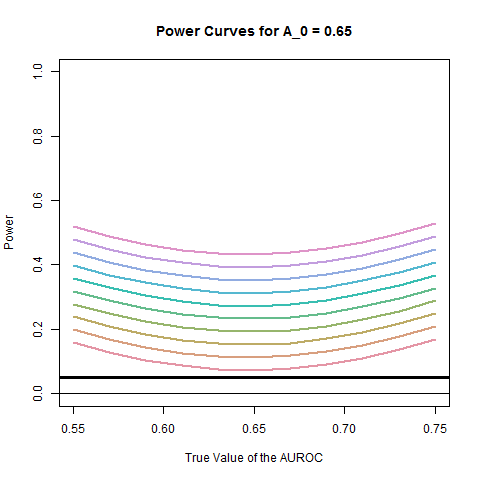
\includegraphics[scale=  0.35]{Figs/Power/fig_power_A_0_65.png}} \\
        
        \subfloat[Power Curves for $H_0: A_0 = 0.75$ ]{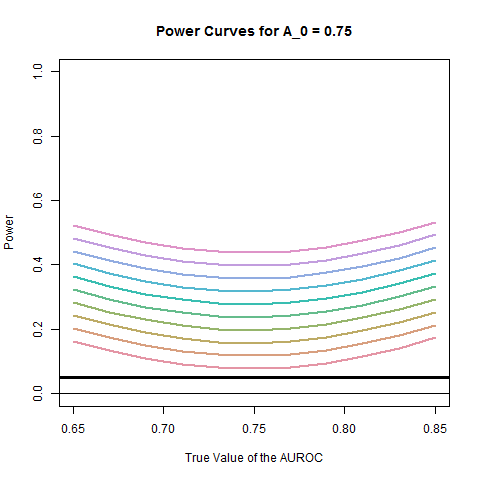
\includegraphics[scale=  0.35]{Figs/Power/fig_power_A_0_75.png}} \\
        
        \subfloat[Power Curves for $H_0: A_0 = 0.85$ ]{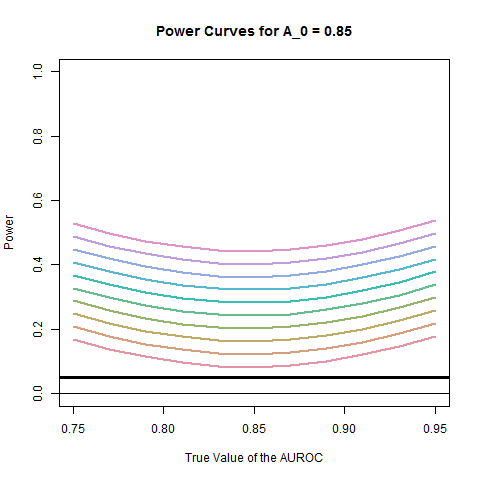
\includegraphics[scale=  0.35]{Figs/Power/fig_power_A_0_85.png}} \\




    \end{tabular}

\end{center}

    \footnotesize

        \textbf{Power Curves: }
        Description goes here.

\end{figure}


%%%%%%%%%%%%%%%%%%%%%%%%%%%%%%%%%%%%%%%%%%%%%%%%%%%%%%%%%%%%%%%%%%%%%%%%%%%%%%%%%%%%%%%%%%%%%%%%%%%%%%%%%%%%%%%




%%%%%%%%%%%%%%%%%%%%%%%%%%%%%%%%%%%%%%%%%%%%%%%%%%%%%%%%%%%%%%%%%%%%%%%%%%%%%%%%%%%%%%%%%%%%%%%%%%%%%%%%%%%%%%%
%%%%%%%%%%%%%%%%%%%%%%%%%%%%%%%%%%%%%%%%%%%%%%%%%%%%%%%%%%%%%%%%%%%%%%%%%%%%%%%%%%%%%%%%%%%%%%%%%%%%%%%%%%%%%%%
